\chapter{Wprowadzenie teoretyczne}
\section{Wykorzystywane terminy}
\label{sec:terminy}
W niniejszej pracy, posłużono się terminologią dystynktywną z punktu widzenia realizacji, rozwoju oraz ewaluacji usług sieciowych. Najbardziej istotne spośród wykorzystywanych terminów wymieniono poniżej. Dla każdego z pojęć, przedstawiono obcojęzyczne tłumaczenie, a także zdefiniowano spójny oraz zwięzły opis.

\subsection*{Usługa sieciowa}
\subsubsection{\textit{Web Service}}
Rodzaj systemu informatycznego cechującego się permanentnym wykonywaniem zdefiniowanych funkcji, tuż po uzyskaniu żądania. Żądanie to, przybiera postać danych, przekazanych w ramach systematycznej struktury. Sposób dostarczenia żądania, jego format, a także metoda odpowiedzi na żądanie, definiowane są poprzez protokół sieciowy z którego korzysta dana usługa.

\subsection*{Interfejs Programowania Aplikacji (API) - OPIS Z INŻ.}
\subsubsection{\textit{Application Programming Interface}}
Zbiór zasad oraz procedur determinujący sposób komunikacji pomiędzy wieloma aplikacjami. Aplikacjami tymi mogą być zarówno programy klienckie (np. strona webowa), jak i serwery danych.

\subsection*{API wykonane w technologii REST - OPIS Z INŻ.}
\subsubsection{\textit{RESTful API}}
Interfejs programowania aplikacji opierający swoją budowę oraz sposób funkcjonowania o zbiór ustalonych reguł. Reguły te, dotyczą między innymi: struktury żądań wysyłanych od klienta do serwera, budowy zasobu odpowiedzi serwera, a także kodów statusów zwracanych z chwilą odpowiedzi w zależności od wykonanej akcji.

\subsection*{Kontroler - OPIS Z INŻ.}
\subsubsection{\textit{Controller}}
Klasa, której zadaniem jest obsłużenie żądania aplikacji klienckiej, weryfikacja jego poprawności, a następnie wywołanie kodu logiki biznesowej w ramach struktur serwisów. Po otrzymaniu rezultatu obliczeń z warstwy logiki biznesowej, odpowiedzialnością metody kontrolera jest zwrócenie przetworzonego zasobu do systemu klienta.

\subsection*{Serwis - OPIS Z INŻ.}
\subsubsection{\textit{Service}}
Klasa, zawierająca metody odpowiedzialne za realizację logiki biznesowej w ramach interfejsu programowania aplikacji. Obiekt tej struktury danych, wywoływany jest bezpośrednio przed metody klas kontrolerów.  

\subsection*{Repozytorium - OPIS Z INŻ.}
\subsubsection{\textit{Repository}}
Struktura danych, wykorzystywana do komunikacji interfejsu API z serwerem bazodanowym. Metody, w ramach klas repozytoriów, operują na modelu danych, przechowywanym w ramach API, a następnie, odwzorowują ten model za pomocą narzędzia ORM, na fizyczną zawartość bazodanową.

\subsection*{Mapper obiektowo-relacyjny (ORM)}
\subsubsection{\textit{Object-relational mapper (ORM)}}
Oprogramowanie, którego głównym zadaniem jest konwersja struktury klas modelu danych do fizycznej organizacji tabel w ramach systemu bazodanowego. Ponadto, mapper obiektowo-relacyjny dostarcza zbiór właściwości oraz metod stanowiących fasadę dla niskopoziomowych procedur dostępu do bazy danych, a także modyfikacji danych w niej zawartych.


\subsection*{Pamięć podręczna}
\subsubsection{\textit{Cache}}
Wydzielony fragment pamięci cechujący się szybkim czasem dostępu, wysoką przepustowością transmisji, a także ograniczonym okresem trwałego przechowywania danych. Pamięć ta, w kontekście webowego interfejsu programowania aplikacji, wykorzystywana jest w celu przechowywania wyników często realizowanych operacji, a także magazynowania uprzednio dostarczonych do klienta fragmentów odpowiedzi na żądania.

\subsection*{Wielowątkowość - OPIS Z INŻ.}
\subsubsection{\textit{Multithreading}}
Technika programowania, zakładająca wykorzystanie wielu odrębnie wykonywanych procesów w ramach jednej aplikacji. W przypadku interfejsu API implementującego tę technikę, każdy z punktów końcowych stanowi osobny wątek, będący częścią składową pojedynczego procesu. Dzięki temu, aplikacja jest dostępna, niezależnie od wywołanych, niekiedy długo trwających zadań.

\subsection*{Algorytm metaheurystyczny}
\subsubsection{\textit{Metaheuristic algorithm}}
Technika projektowania algorytmów nie zapewniających gwarancji uzyskania optimum dla rozważanego problemu, jednakże pozwalająca na zbudowanie systemu, dostarczającego rozwiązanie złożonego zagadnienia w akceptowalnym czasie, a także uzyskiwanego przy wykorzystaniu akceptowalnej ilości zasobów sprzętowych. Algorytm metaheurystyczny, poza konwencjonalnymi regułami stosowanymi w ramach standardowych wzorców programowania, implementuje reguły rozwiązywania problemów oparte na losowości, bądź też wywnioskowane na podstawie zjawisk fizycznych.

\subsection*{Punkt końcowy usługi sieci Web - OPIS Z INŻ.}
\subsubsection{\textit{Endpoint}}
Metoda klasy kontrolera, uruchamiana w momencie określenia żądania klienta. Do każdego z punktów końcowych, przypisany jest adres wywołania, zbiór wymaganych parametrów, a także obsługiwany typ metody protokołu hipertekstowego. Dzięki temu, bazując na strukturze otrzymanego żądania, interfejs API jest w stanie stwierdzić który z punktów końcowych powinien zostać wywołany.

\subsection*{Żądanie realizowane w ramach usługi protokołu hipertekstowego}
\subsubsection{\textit{HTTP Request}}
Struktura danych, wysyłana od aplikacji klienckiej (tj. aplikacji internetowej, przeglądarki, czy też programu klienta HTTP) w kierunku usługi sieciowej. Żądanie protokołu hipertekstowego charakteryzuje się jednoznacznie zdefiniowaną strukturą, uwzględniającą m.in. unikalny identyfikator zasobu, listę zdefiniowanych nagłówków, ciało żądania oraz jedną z dziewięciu dopuszczalnych metod HTTP. 

\subsection*{Odpowiedź usługi protokołu hipertekstowego}
\subsubsection{\textit{HTTP Response}}
Struktura danych, wysyłana przez usługę sieciową w kierunku aplikacji klienckiej. Odpowiedź HTTP, ma na celu poinformowanie klienta serwisu webowego o statusie realizacji, wysłanego przez niego uprzednio żądania. Podstawowymi elementami odpowiedzi usługi protokołu hipertekstowego są: ciało odpowiedzi (zdefiniowane najczęściej z wykorzystaniem notacji JSON lub języka XML), kod odpowiedzi (liczba determinująca stan wykonania żądania), a także zbiór informacji nagłówkowych dotyczących typu danych zawartych w odpowiedzi, czy też fizycznych informacji o serwerze usługi sieciowej.

\subsection*{Kod odpowiedzi usługi protokołu hipertekstowego}
\subsubsection{\textit{HTTP Response Code}}
Liczba determinująca status realizacji żądania wysłanego przez aplikację kliencką. Kod odpowiedzi stanowi jedną z wymaganych składowych dotyczących standardowego rezultatu zwracanego w ramach usługi opartej o protokół hipertekstowy. Wyróżnić możemy pięć kategorii kodów odpowiedzi, niosących ze sobą odmienną informacje. Kategoriami tymi są: kody informacyjnej odpowiedzi (100-199), kody poprawnej odpowiedzi (200-299), kody wiadomości o przekierowaniu (300-399), kody błędu aplikacji klienckiej (400-499), oraz kody błędu aplikacji serwerowej (500-599).

\subsection*{Czas odpowiedzi usługi protokołu hipertekstowego}
\subsubsection{\textit{HTTP Response Time}}
Wyrażony w milisekundach, przedział czasu od momentu otrzymania żądania wygenerowanego przez aplikację kliencką, do chwili zwrócenia rezultatu wykonywanych przez usługę sieciową obliczeń. Liczba ta, stanowi jedną z wartości pomiarowych, w kontekście efektywności działania interfejsu programowania aplikacji.  

\subsection*{Obiektowa notacja JavaScript (JSON) - OPIS Z INŻ.}
\subsubsection{\textit{JavaScript Object Notation}}
Niezależny od języka programowania format prezentacji, definicji oraz wymiany danych w formie obiektów. Powszechnie stosowany jako sposób generowania ciała żądania wysyłanego do interfejsu API, a także odpowiedzi od niego uzyskiwanej.

\subsection*{Testy wzorcowe}
\subsubsection{\textit{Benchmark}}
Rodzaj ewaluacji oprogramowania, której zadaniem jest określenie referencyjnego poziomu wydajności dla testowanego systemu. Metryki, uzyskane w ramach testów wzorcowych, mogą zostać wykorzystane jako wartości ograniczeń względem testów obciążeniowych oraz przeciążeniowych. 

\subsection*{Testy dymne}
\subsubsection{\textit{Smoke testing}}
Metoda testowania oprogramowania, której celem jest sprawdzenie poprawności funkcjonowania poszczególnych elementów systemu. Testy dymne, wykonywane są przed testami wydajnościowymi, po to aby upewnić się co do braku błędów implementacyjnych w ramach analizowanego oprogramowania.

\subsection*{Testy wydajności podstawowej}
\subsubsection{\textit{Baseline performance testing}}
Metoda ewaluacji oprogramowania, pozwalająca na weryfikację działania systemu w warunkach analogicznych do realiów standardowego działania. Na podstawie testów wydajności podstawowej, określić można wartości metryk, które będą miały zastosowanie jako punkt odniesienia dla kolejnych rodzajów testów. Ponadto, wykorzystując standard pomiaru wydajności aplikacji internetowych (taki jak np. APDEX), wartości uzyskane w ramach ewaluacji podstawowych, mogą posłużyć w celu określenia punktów satysfakcji, tolerancji oraz frustracji.

\subsection*{Testy obciążeniowe}
\subsubsection{\textit{Load testing}}
Rodzaj testów, które mają na celu określenie maksymalnego poziomu natężenia operacji, jakie mogą być generowane w kierunku oprogramowania. W kontekście niniejszej pracy, operacjami tymi są żądania wysyłane do interfejsu programowania aplikacji. Kluczowym aspektem testu obciążeniowego jest zdefiniowanie progu obciążenia aplikacji, powyżej którego system jest nie w stanie generować poprawnych odpowiedzi w akceptowalnym czasie.

\subsection*{Testy przeciążeniowe}
\subsubsection{\textit{Stress testing}}
Metoda ewaluacji oprogramowania, w ramach której natężenie operacji generowanych w kierunku testowanego oprogramowania zwiększone jest ponad ustalony próg tolerancji. Celem testu przeciążeniowego jest obserwacja sposobu działania systemu, w momencie, w którym nie jest on w stanie przetwarzać otrzymywanych żądań w sposób poprawny.

\subsection*{Asercja}
\subsubsection{\textit{Assertion}}
Wyrażenie typu prawda/fałsz, zdefiniowane w dowolnym miejscu programu, które przyjmuje wartość prawdziwą w momencie spełnienia hipotezy zawartej w ramach określonego przypadku testowego. Praktyczne podejście do procesu testowania funkcjonalności oprogramowania, sprowadza się do definiowania hipotez oraz ciągów operacji w kontekście przypadków testowych, a następnie weryfikacji tych hipotez z wykorzystaniem asercji.

\section{Interfejsy programowania aplikacji}
Webowy interfejs programowania aplikacji to usługa sieciowa, której celem jest realizacja zadań zleconych przez oprogramowanie klienta. Zadania te, dotyczą operacji wykonywanych w kontekście określonych zasobów. Wyróżnić możemy operacje zwane zapytaniami (tj. dotyczące pozyskiwania danych z ich źródeł), a także komendami (tj. związane z wykonywaniem operacji na danych).

Interfejsy API, budowane są z wykorzystaniem protokołu HTTP, dlatego też w ich kontekście możemy mówić o komunikacji bezstanowej definiującej pojęcia żądania oraz odpowiedzi. W związku z charakterystyką protokołu hipertekstowego, zarówno żądanie jak i odpowiedź cechuje się regularną strukturą zawierającą predefiniowane elementy.

Żądanie protokołu http wysyłane jest od aplikacji klienta do interfejsu API. Podstawową składową tego polecenia stanowi unikalny identyfikator zasobu URI (\textit{ang. Uniform Resource Identifier}), na podstawie którego możliwe jest określenie fragmentu dziedziny obsługiwanego modelu danych. Informacja ta jednak, nie jest wystarczająca w kontekście realizacji jednej z funkcjonalności, zdefiniowanych w ramach API. Żądanie klienta, musi zostać uzupełnione o jedną z dziewięciu ustalonych metod http, obsługiwaną wersję protokołu, a także zbiór linii nagłówkowych. Opcjonalnie, informacja wysyłana w kierunku interfejsu, może zostać wzbogacona o zawartość tekstową określaną ciałem żądania (\textit{ang. Request body}). Taki zbiór informacji, pozwala na jednoznaczną identyfikacje fragmentu kodu programu, który ma zostać wykonany wewnątrz interfejsu programowania aplikacji. W tabelach \ref{tab:metody-http} oraz \ref{tab:naglowki-zadanie} przedstawiono kolejno listę zdefiniowanych metod protokołu hipertekstowego wraz z wyjaśnieniem ich przeznaczenia, a także zbiór najczęściej wykorzystywanych linii nagłówkowych, w kontekście realizacji żądań.

\begin{table}[htbp] \small
\centering
\caption{Zbiór dozwolonych metod protokołu hipertekstowego}
\label{tab:metody-http}
\begin{tabularx}{\linewidth}{|p{3cm}|X|} \hline\
Nazwa metody & Opis \\ \hline\hline
GET & Pozyskanie danych dotyczących pojedynczej instancji określonego zasobu lub grupy instancji z opcjonalnym uwzględnieniem warunków kwalifikacji poszczególnej instancji do grupy. \\ \hline
POST & Definiowanie nowej instancji dotyczącej określonego typu zasobu. Przy zastosowaniu metody POST, wymagane jest zdefiniowanie ciała żądania, jako części składowej generowanej instrukcji. \\ \hline
PUT & Aktualizacja pełni zawartości instancji występującej w ramach odwołania się do określonego zasobu. Przy zastosowaniu metody PUT, wymagane jest zdefiniowanie ciała żądania, jako części składowej generowanej instrukcji. \\ \hline
DELETE & Usunięcie istniejącej instancji dotyczącej określonego typu zasobu. \\ \hline
PATCH & Aktualizacja fragmentu zawartości instancji występującej w ramach odwołania się do określonego zasobu. Przy zastosowaniu metody PATCH, wymagane jest zdefiniowanie ciała żądania, jako części składowej generowanej instrukcji. \\ \hline
HEAD & Pozyskanie zbioru linii nagłówkowych, które byłyby dostarczone wraz z ciałem odpowiedzi w ramach żądania wykorzystującego metodę GET. Wygenerowanie żądania HEAD umożliwia określenie charakteru danych, przed ich ewentualnym pozyskaniem. \\ \hline
OPTIONS & Pozyskanie informacji dotyczących charakterystyki oraz struktury serwera. Definiując żądanie typu OPTIONS, klient może dowiedzieć się o dopuszczalnych metodach HTTP obsługiwanych przez serwer, czy też uzyskać informacje o nazwie serwera oraz wykorzystywanym systemie operacyjnym. \\ \hline
CONNECT & Ustanowienie dwukierunkowej komunikacji pomiędzy klientem a serwerem. W przypadku realizacji komunikacji szyfrowanej, żądanie typu CONNECT pozwala na zestawienie zabezpieczonego tunelu pomiędzy hostami. \\ \hline
TRACE & Wygenerowanie komunikatu diagnostycznego w ramach pętli zwrotnej, którego celem jest osiągnięcie każdego z hostów, biorących udział w komunikacji. \\ \hline
\end{tabularx}
\end{table}

\begin{table}[htbp] \small
\centering
\caption{Zbiór najczęściej wykorzystywanych linii nagłówkowych w kontekście żądania protokołu hipertekstowego}
\label{tab:naglowki-zadanie}
\begin{tabularx}{\linewidth}{|p{5cm}|X|X|} \hline\
Linia nagłówkowa & Znaczenie & Dopuszczalna zawartość \\ \hline\hline
accept & Typ zawartości, którą jest w stanie przetwarzać aplikacja kliencka & Identyfikator typu MIME (\textit{ang. Multipurpose Internet Mail Extensions}) lub zapis */* oznaczający dowolną zawartość  \\ \hline
accept-encoding & Sposób kodowania znaków, rozumiany przez stronę klienta & Zbiór formatów kodowania zdefiniowany w ramach rejestru formatów IANA\\ \hline
accept-language & Język naturalny, preferowany przez stronę kliencką & Pojedyncza wartość reprezentująca określony kraj lub region, bądź też lista niniejszych wartości wraz z parametrem istotności poszczególnego kodu lokalizacji\\ \hline
content-length & Długość ciała żądania wyrażona w bajtach & Liczba naturalna\\ \hline
content-type & Format zawartości ciała żądania & Identyfikator typu MIME wraz ze sposobem kodowania wiadomości\\ \hline
cookie & Zbiór informacji pozwalających na wprowadzenie oraz utrzymanie stanowego charakteru transmisji & Zestaw par klucz-wartość, gdzie klucz jest wartością tekstową, a wartość przyjmuje postać dowolną\\ \hline
origin & Informacja determinująca pochodzenie żądania & Ciąg tekstowy składający się z nazwy protokołu, nazwy hosta oraz numeru portu\\ \hline
user-agent & Specyfikacja techniczna oprogramowania klienta & Ciąg znaków zawierający informacje o nazwie produktu, jego wersji, platformie sprzętowej, czy też systemie operacyjnym \\ \hline
\end{tabularx}
\end{table}

Po wykonaniu kodu programu przypisanego do określonego rodzaju polecenia generowanego przez aplikacje kliencką, z interfejsu programowania aplikacji zwracana jest odpowiedź na żądanie (\textit{ang. HTTP response}). Analogicznie do instrukcji realizacji danej czynności, także odpowiedź dotycząca statusu jej wykonania jest ustrukturyzowana zgodnie z wytycznymi zawartymi w definicji protokołu hipertekstowego. W ramach rezultatu zwróconego przez API wyróżnić należy: adres docelowy klienta, kod statusu, ciało odpowiedzi, a także zbiór linii nagłówkowych. Informacja zawarta w ramach kodu statusu, determinuje powodzenie realizowanej operacji, a treść dostarczanych linii nagłówkowych, może zostać wykorzystana w celu wnioskowania o charakterystyce odbywającej się komunikacji. Ciało odpowiedzi powinno zawierać dane dotyczące definiowanego w ramach identyfikatora żądania zasobu, w przypadku żądań wykorzystujących metodę GET. W kontekście pozostałych żądań, zgodnie z wytycznymi dokumentów RFC (\textit{ang. Request For Comments}) o numerach 7230 do 7237, powinno ono posiadać charakter informacji pomocniczej, bądź też pozostać puste. W ramach tabel \ref{tab:naglowki-odpowiedz} oraz \ref{tab:kody-odpowiedzi}, wymienione zostały kolejno: zbiór najczęściej zwracanych linii nagłówkowych w kontekście odpowiedzi na żądanie, a także przedziały liczbowe dla kodów statusu odpowiedzi, wraz z ich semantyką.

\begin{table}[htbp] \small
\centering
\caption{Zbiór najczęściej zwracanych linii nagłówkowych w kontekście odpowiedzi protokołu hipertekstowego}
\label{tab:naglowki-odpowiedz}
\begin{tabularx}{\linewidth}{|p{5cm}|X|X|} \hline\
Linia nagłówkowa & Znaczenie & Dopuszczalna zawartość \\ \hline\hline
access-control-allow-credentials & Określenie, czy odpowiedź serwera ma być osiągalna z kodu JavaScript aplikacji klienckiej, w momencie gdy nagłówek żądania dotyczący poświadczeń, zezwala na ich dołączenie & Wartość prawda/fałsz \\ \hline
access-control-allow-origin & Informacja dotycząca pochodzenia klienta, który może ubiegać się o otrzymanie odpowiedzi od serwera & adres hosta klienckiego lub symbol gwiazdki oznaczający zezwolenie dla wszystkich hostów\\ \hline
cache-control & Dane konfiguracyjne dotyczące obsługi pamięci podręcznej & Zbiór par klucz-wartość określających zachowanie pamięci cache w kontekście określonej komunikacji\\ \hline
content-length & Długość ciała odpowiedzi wyrażona w bajtach & Liczba naturalna\\ \hline
content-type & Format zawartości ciała odpowiedzi & Identyfikator typu MIME wraz ze sposobem kodowania wiadomości\\ \hline
cross-origin-resource-policy & Polecenie ignorowania żądań realizowanych pomiędzy źródłami bądź witrynami w kontekście określonego zasobu  & Wartość prawda/fałsz \\ \hline
expires & Data wygaśnięcia ważności niniejszej odpowiedzi & Określona data \\ \hline
server & Nazwa hosta dostarczającego odpowiedź klientowi & Ciąg znaków \\ \hline
\end{tabularx}
\end{table}

\begin{table}[htbp] \small
\centering
\caption{Zbiór kodów statusu odpowiedzi protokołu hipertekstowego}
\label{tab:kody-odpowiedzi}
\begin{tabularx}{\linewidth}{|p{4cm}|X|X|} \hline\
Przedział liczbowy & Semantyka w kontekście odpowiedzi\\ \hline\hline
100 - 199 & Zbiór kodów informacyjnych - żądanie jest aktualnie przetwarzanie\\ \hline
200 - 299 & Zbiór kodów poprawnej odpowiedzi - wystosowane żądanie zostało zrealizowane poprawnie \\ \hline
300 - 399 & Zbiór kodów przekierowań - istnieć może wiele akceptowalnych odpowiedzi dla żądania bądź realizacja określonej operacji wymusza odwołanie się pod adres identyfikujący odmienny zasób \\ \hline
400 - 499 & Zbiór kodów błędu po stronie klienta - wygenerowane żądanie zawiera błędy, oczekiwany zasób nie istnieje, klient nie jest uwierzytelniony lub nie posiada określonego poziomu uprawnień \\ \hline
500 - 599 & Zbiór kodów błędu po stronie serwera - pomimo poprawnej struktury wygenerowanego żądania, serwer nie jest w stanie zrealizować przydzielonej mu operacji\\ \hline
\end{tabularx}
\end{table}

Przedstawiony w niniejszy sposób interfejs programowania aplikacji scharakteryzować należy jako deterministyczny system wejściowo-wyjściowy. Ponadto, należy zauważyć, że w ramach systemu tego, występuje zjawisko inercji, powodowane koniecznością realizacji zdefiniowanego w ramach API kodu programu. Na podstawie tego założenia, ewaluację działania oraz wydajności interfejsu programowania aplikacji przeprowadzić można poprzez wprowadzanie określonego wejścia (tj. generowanie żądania) oraz obserwację wartości zwróconej na wyjściu (tj. uzyskana odpowiedź).

\subsection*{Proces przetwarzania żądania wewnątrz interfejsu API}
Po uzyskaniu żądania otrzymanego od strony klienta, zadaniem interfejsu programowania aplikacji jest wybór określonej klasy kontrolera, a także zawartej w niej metody. Każda z klas kontrolerów stworzona jest w celu obsługi operacji związanych z konkretnym zasobem, a poszczególna metoda tej klasy implementuje zachowanie które ma zostać wywołane w kontekście dostarczonego typu oraz identyfikatora polecenia.

Wewnątrz metody klasy warstwy kontrolerów, wywoływane zostają operacje zdefiniowane w usługach warstwy biznesowej. Usługi te, realizowane mogą być zarówno wewnątrz api jak i stanowić odrębny system internetowy. Klasy warstwy logiki biznesowej, zwane serwisami, złożone są z metod, których głównym celem jest weryfikacja poprawności otrzymanych informacji w kontekście obsługiwanych zasobów, a także pozyskiwanie danych oraz wykonywanie operacji na nich, poprzez odwoływanie się do metod warstwy dostępu do danych.

Zbiór klas warstwy dostępu do danych, stanowi ostatni z logicznych poziomów, definiowanych w ramach architektury API. Fragmenty kodu zdefiniowane w tej warstwie, zwane repozytoriami, mają za zadanie obsłużyć komunikację pomiędzy interfejsem programowania aplikacji, a określonym źródłem danych. Ponadto, metody klas repozytoriów, dostarczają warstwie logiki biznesowej interfejs operacji na danych. Dzięki temu, żądanie może być przetwarzane od warstw najwyższych (tj. warstwy kontrolerów) do warstwy najniższej (tj. warstwy dostępu do danych), natomiast odpowiedź na żądanie jest konsolidowana w kierunku odwrotnym. Na ilustracji \ref{fig:architektura-api} przedstawiono przepływ informacji wewnątrz interfejsu API, od momentu wygenerowania żądania do chwili uzyskania odpowiedzi.

\begin{figure}[ht]
 \centering
  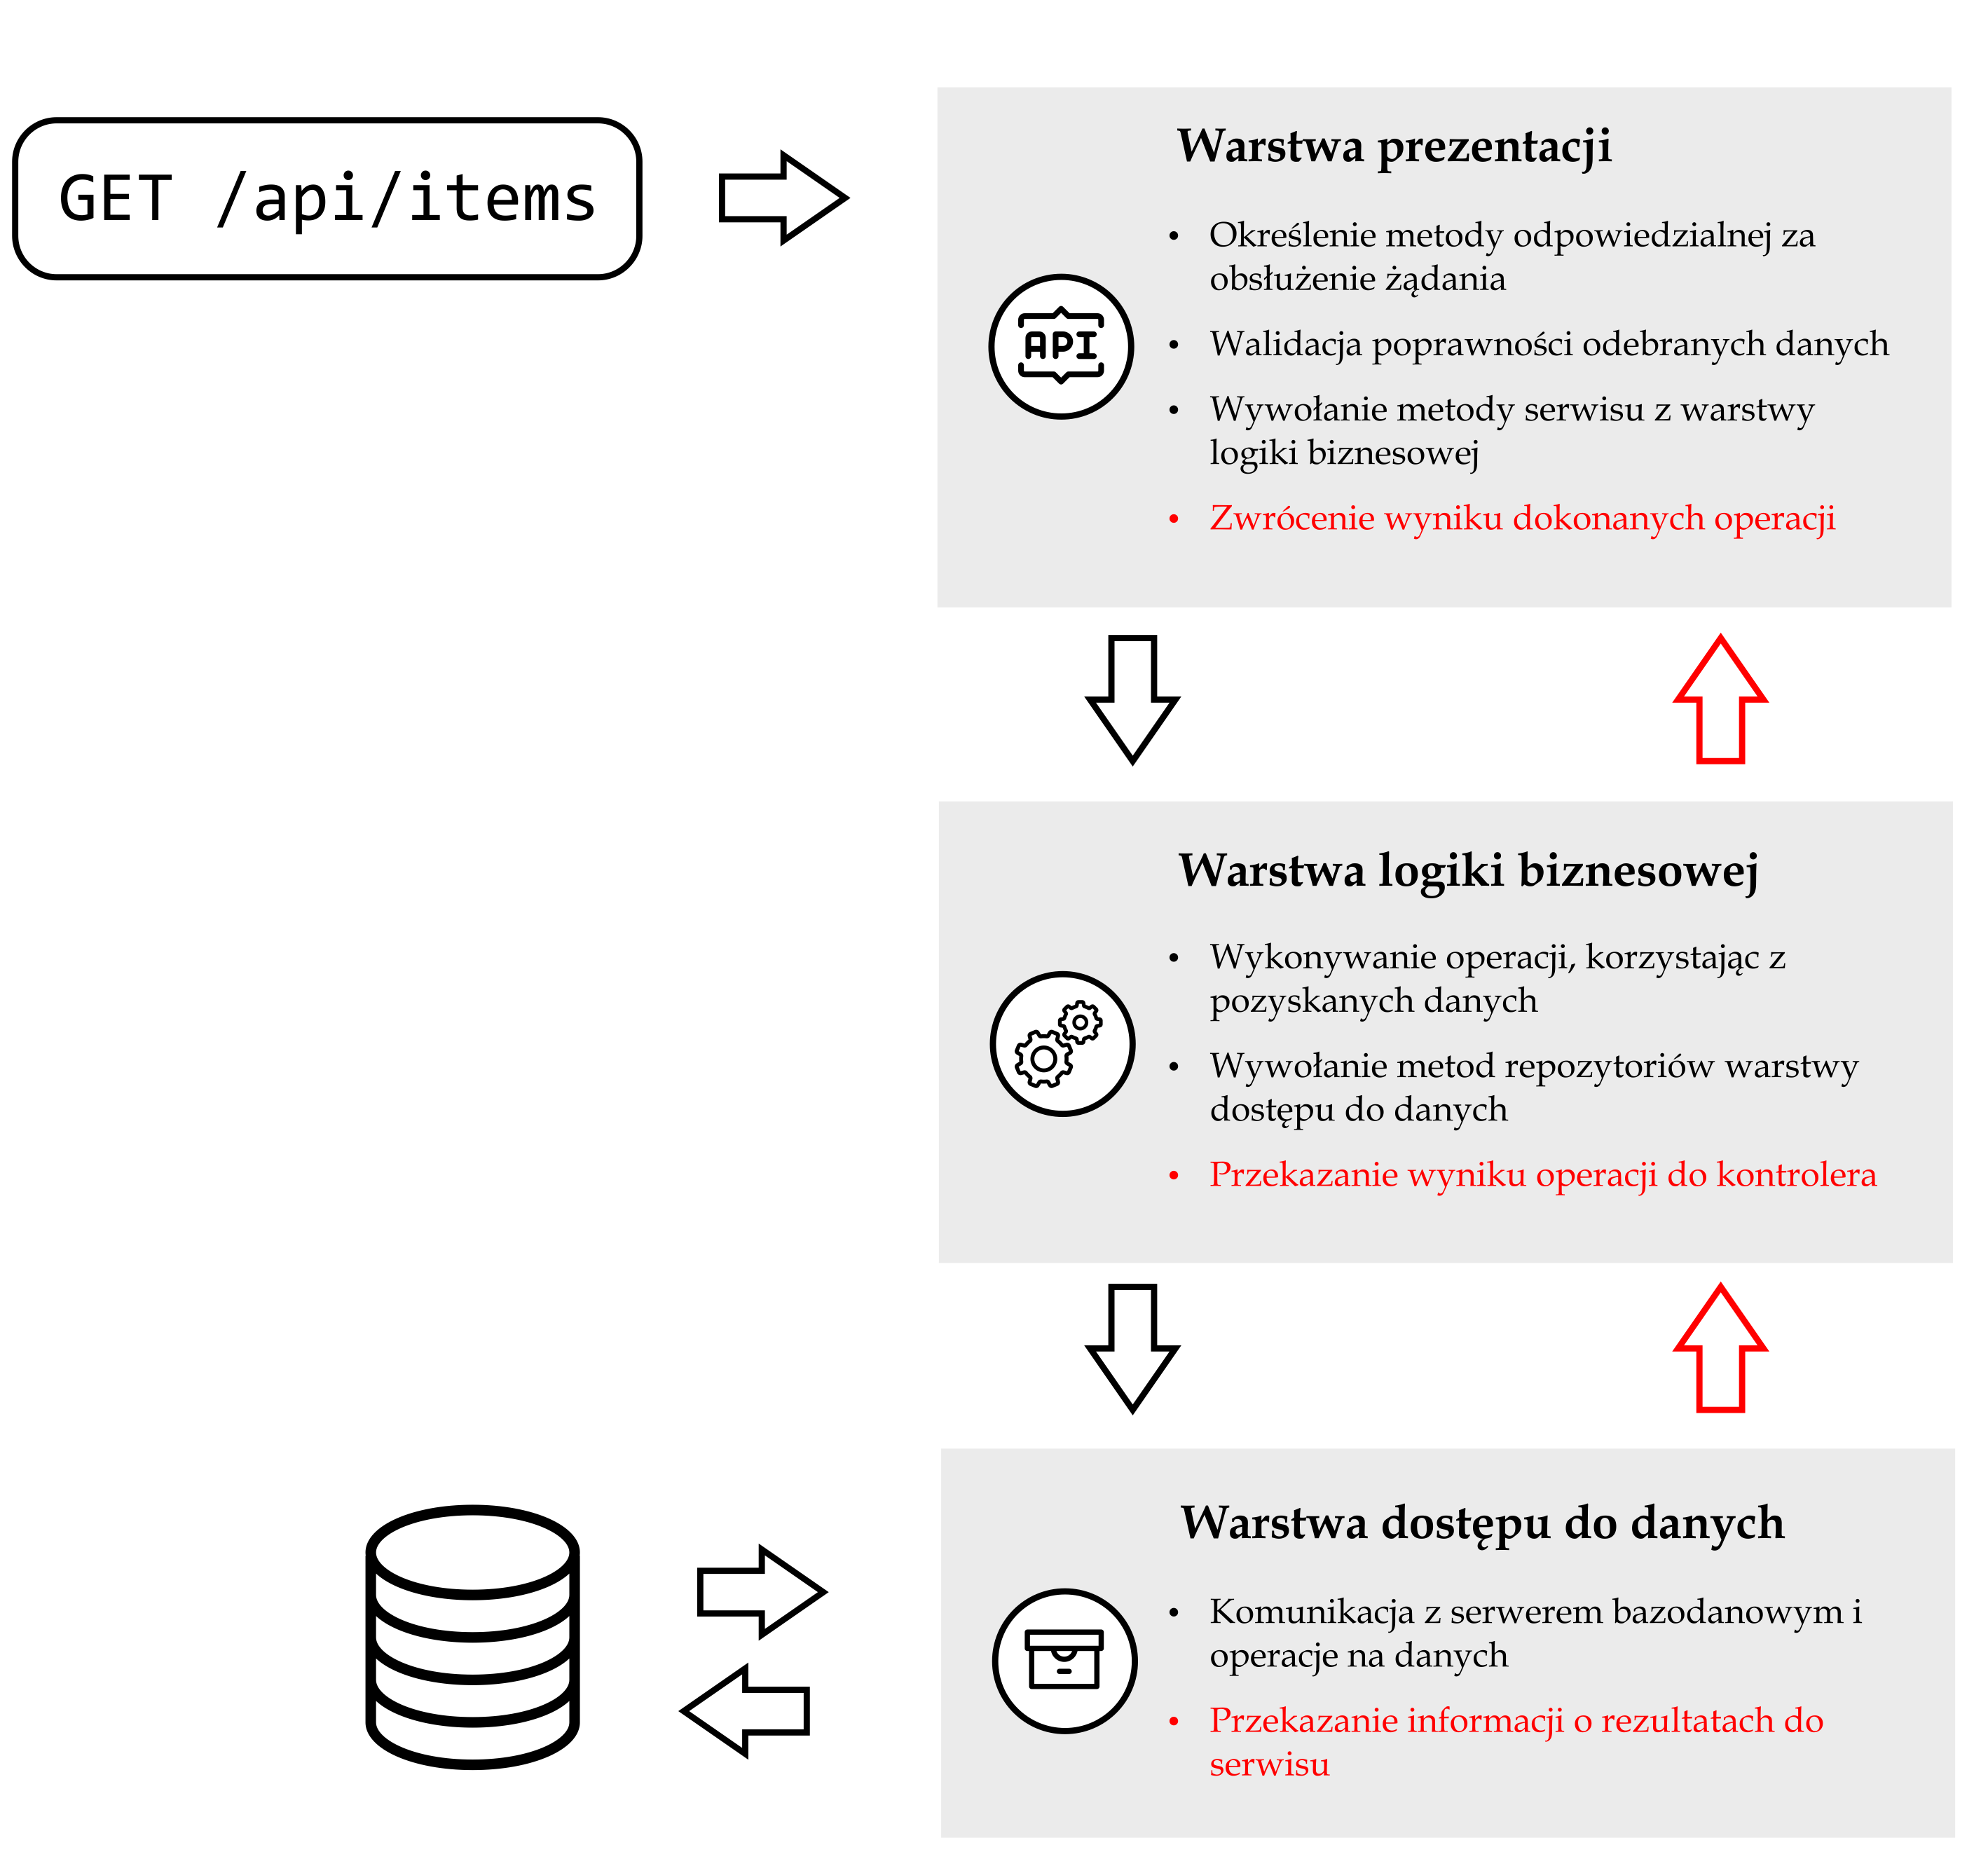
\includegraphics[width=0.6\linewidth]{rys03/architektura-api}
 \caption{Proces przetwarzania żądania wewnątrz interfejsu API}
 \label{fig:architektura-api}
\end{figure}
 
\subsection*{Mapowanie obiektowo-relacyjne oraz podejście Code-First}
W celu uproszczenia procesu pozyskiwania oraz modyfikacji danych z zewnętrznych źródeł, a także unifikacji sposobu interakcji z nimi, w ramach interfejsów programowania aplikacji, powszechnie wykorzystywane jest oprogramowanie zwane mapperem obiektowo-relacyjnym (\textit{ang. Object-Relational Mapper}). Założeniem oprogramowania tego, jest zdefiniowanie warstwy abstrakcji pomiędzy interfejsem programowania aplikacji a językiem programowania bądź zbiorem poleceń, wykorzystywanym w ramach obsługi źródła danych.

Podstawowe składowe oprogramowania typu ORM to jednolity interfejs operacji na zbiorze danych, klasy kontekstu bazodanowego, a także metody obsługi komunikacji z bazą danych.

Dzięki wprowadzeniu jednolitego interfejsu operacji na danych, niezależnie od źródła informacji z jakim komunikuje się API, wydanie konkretnego polecenia do dowolnego systemu bazodanowego równoznaczne jest z każdorazowym wywołaniem funkcji o takiej samej sygnaturze. Stosując takie podejście, konstruktor interfejsu programowania aplikacji nie staje się uzależniony od źródła danych z którym pracuje. Ponadto, istnieje możliwość zamiany lub połączenia dodatkowego systemu bazodanowego, a operacja ta, nie wpływa w jakikolwiek sposób na działanie interfejsu API. Niniejsza zależność została zilustrowana na rysunku \ref{fig:orm-wyjasnienie}

\begin{figure}[ht]
 \centering
  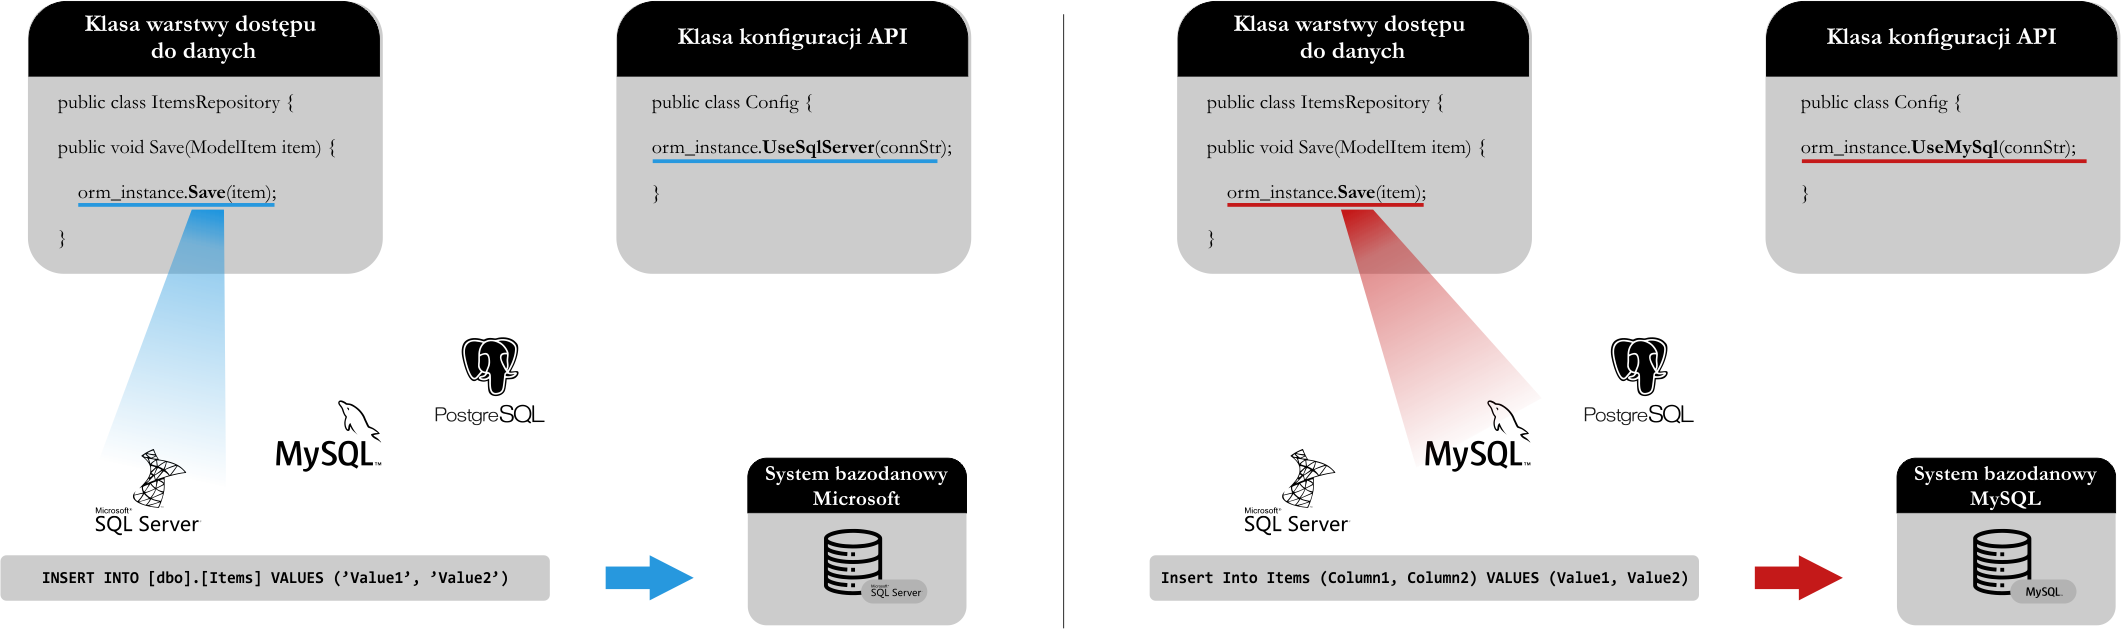
\includegraphics[width=1\linewidth]{rys03/orm-wyjasnienie}
 \caption{Zasada działania oprogramowania mappera obiektowo-relacyjnego w kontekście jednolitego interfejsu operacji na zbiorze danych}
 \label{fig:orm-wyjasnienie}
\end{figure}

Dystynktywnym elementem oprogramowania mappera obiektowo-relacyjnego jest klasa kontekstu bazodanowego. Klasa ta, jest kontenerem struktur w ramach których wyróżnić możemy zbiory elementów modelu danych, a także konfigurację poszczególnych ich właściwości. Podstawową ideą omawianej konwersji dziedziny obiektowej do domeny relacyjnej jest zdefiniowanie zbioru klas, opisujących wykorzystywane zasoby, a następnie odwzorowanie ich w relacyjnym modelu danych, obsługiwanym przez wybrany system bazodanowy. Klasa kontekstu pozwala na określenie, które spośród struktur danych zdefiniowanych w ramach API powinny zostać rzutowane na obiekty tabel generowanych w obrębie bazy danych. Ponadto, dla właściwości każdej z klas modelu danych, zdefiniować należy konfigurację, która zostanie przetransformowana do modelu relacyjnego. W zakresie klasy kontekstu bazy danych, opisywane są także relacje, jakie mają zostać wygenerowane pomiędzy poszczególnymi elementami modelu.

W celu nawiązania, utrzymania, a także zakończenia komunikacji z zewnętrznym źródłem danych, oprogramowanie ORM wykorzystuje klasy zwane konektorami. Klasy te, dostarczają przejrzysty interfejs obsługi połączenia, który następnie jest opakowywany w zunifikowany interfejs, dostępny bezpośrednio dla twórcy API.

\subsection*{Uwierzytelnienie oraz autoryzacja}
Proces uwierzytelnienia oraz autoryzacji użytkownika odwołującego się do interfejsu programowania aplikacji, przedstawić należy w trzech następujących krokach.

Pierwszym z nich, jest wygenerowanie żądania odwołującego się do punktu końcowego odpowiedzialnego za obsługę uwierzytelnienia wewnątrz API. Żądanie to, musi posiadać ciało, zawierające informacje poświadczające o konkretnymi użytkowniku. Najczęściej, informacją tą, jest nazwa użytkownika oraz hasło.

Następnie, dostarczone referencje są analizowane przez mechanizmy uwierzytelniania implementowane w ramach API. W rezultacie tych operacji, zwrócona zostaje pozytywna odpowiedź zawierająca token autoryzujący bądź też negatywna, posiadająca w sobie informację o błędzie uwierzytelnienia klienta.

Strona kliencka może autoryzować dysponowane operacje przed interfejsem programowania aplikacji, uwzględniając w ramach linii nagłówkowej żądania token uwierzytelniający. Dostarczona w ten sposób informacja, pozwala na identyfikację użytkownika w ramach interfejsu API, a także na określenie przypisanego użytkownikowi poziomu uprawnień. W ramach struktury tokenu, zawarta jest także informacja o jego czasie ważności, dlatego też, procedura uwierzytelniania musi być regularnie ponawiana.

Na rysunku \ref{fig:uwierzytelnianie-autoryzacja}, zilustrowany został proces uwierzytelnienia i autoryzacji aplikacji klienta przez interfejsem programowania aplikacji. 

\begin{figure}[ht]
 \centering
  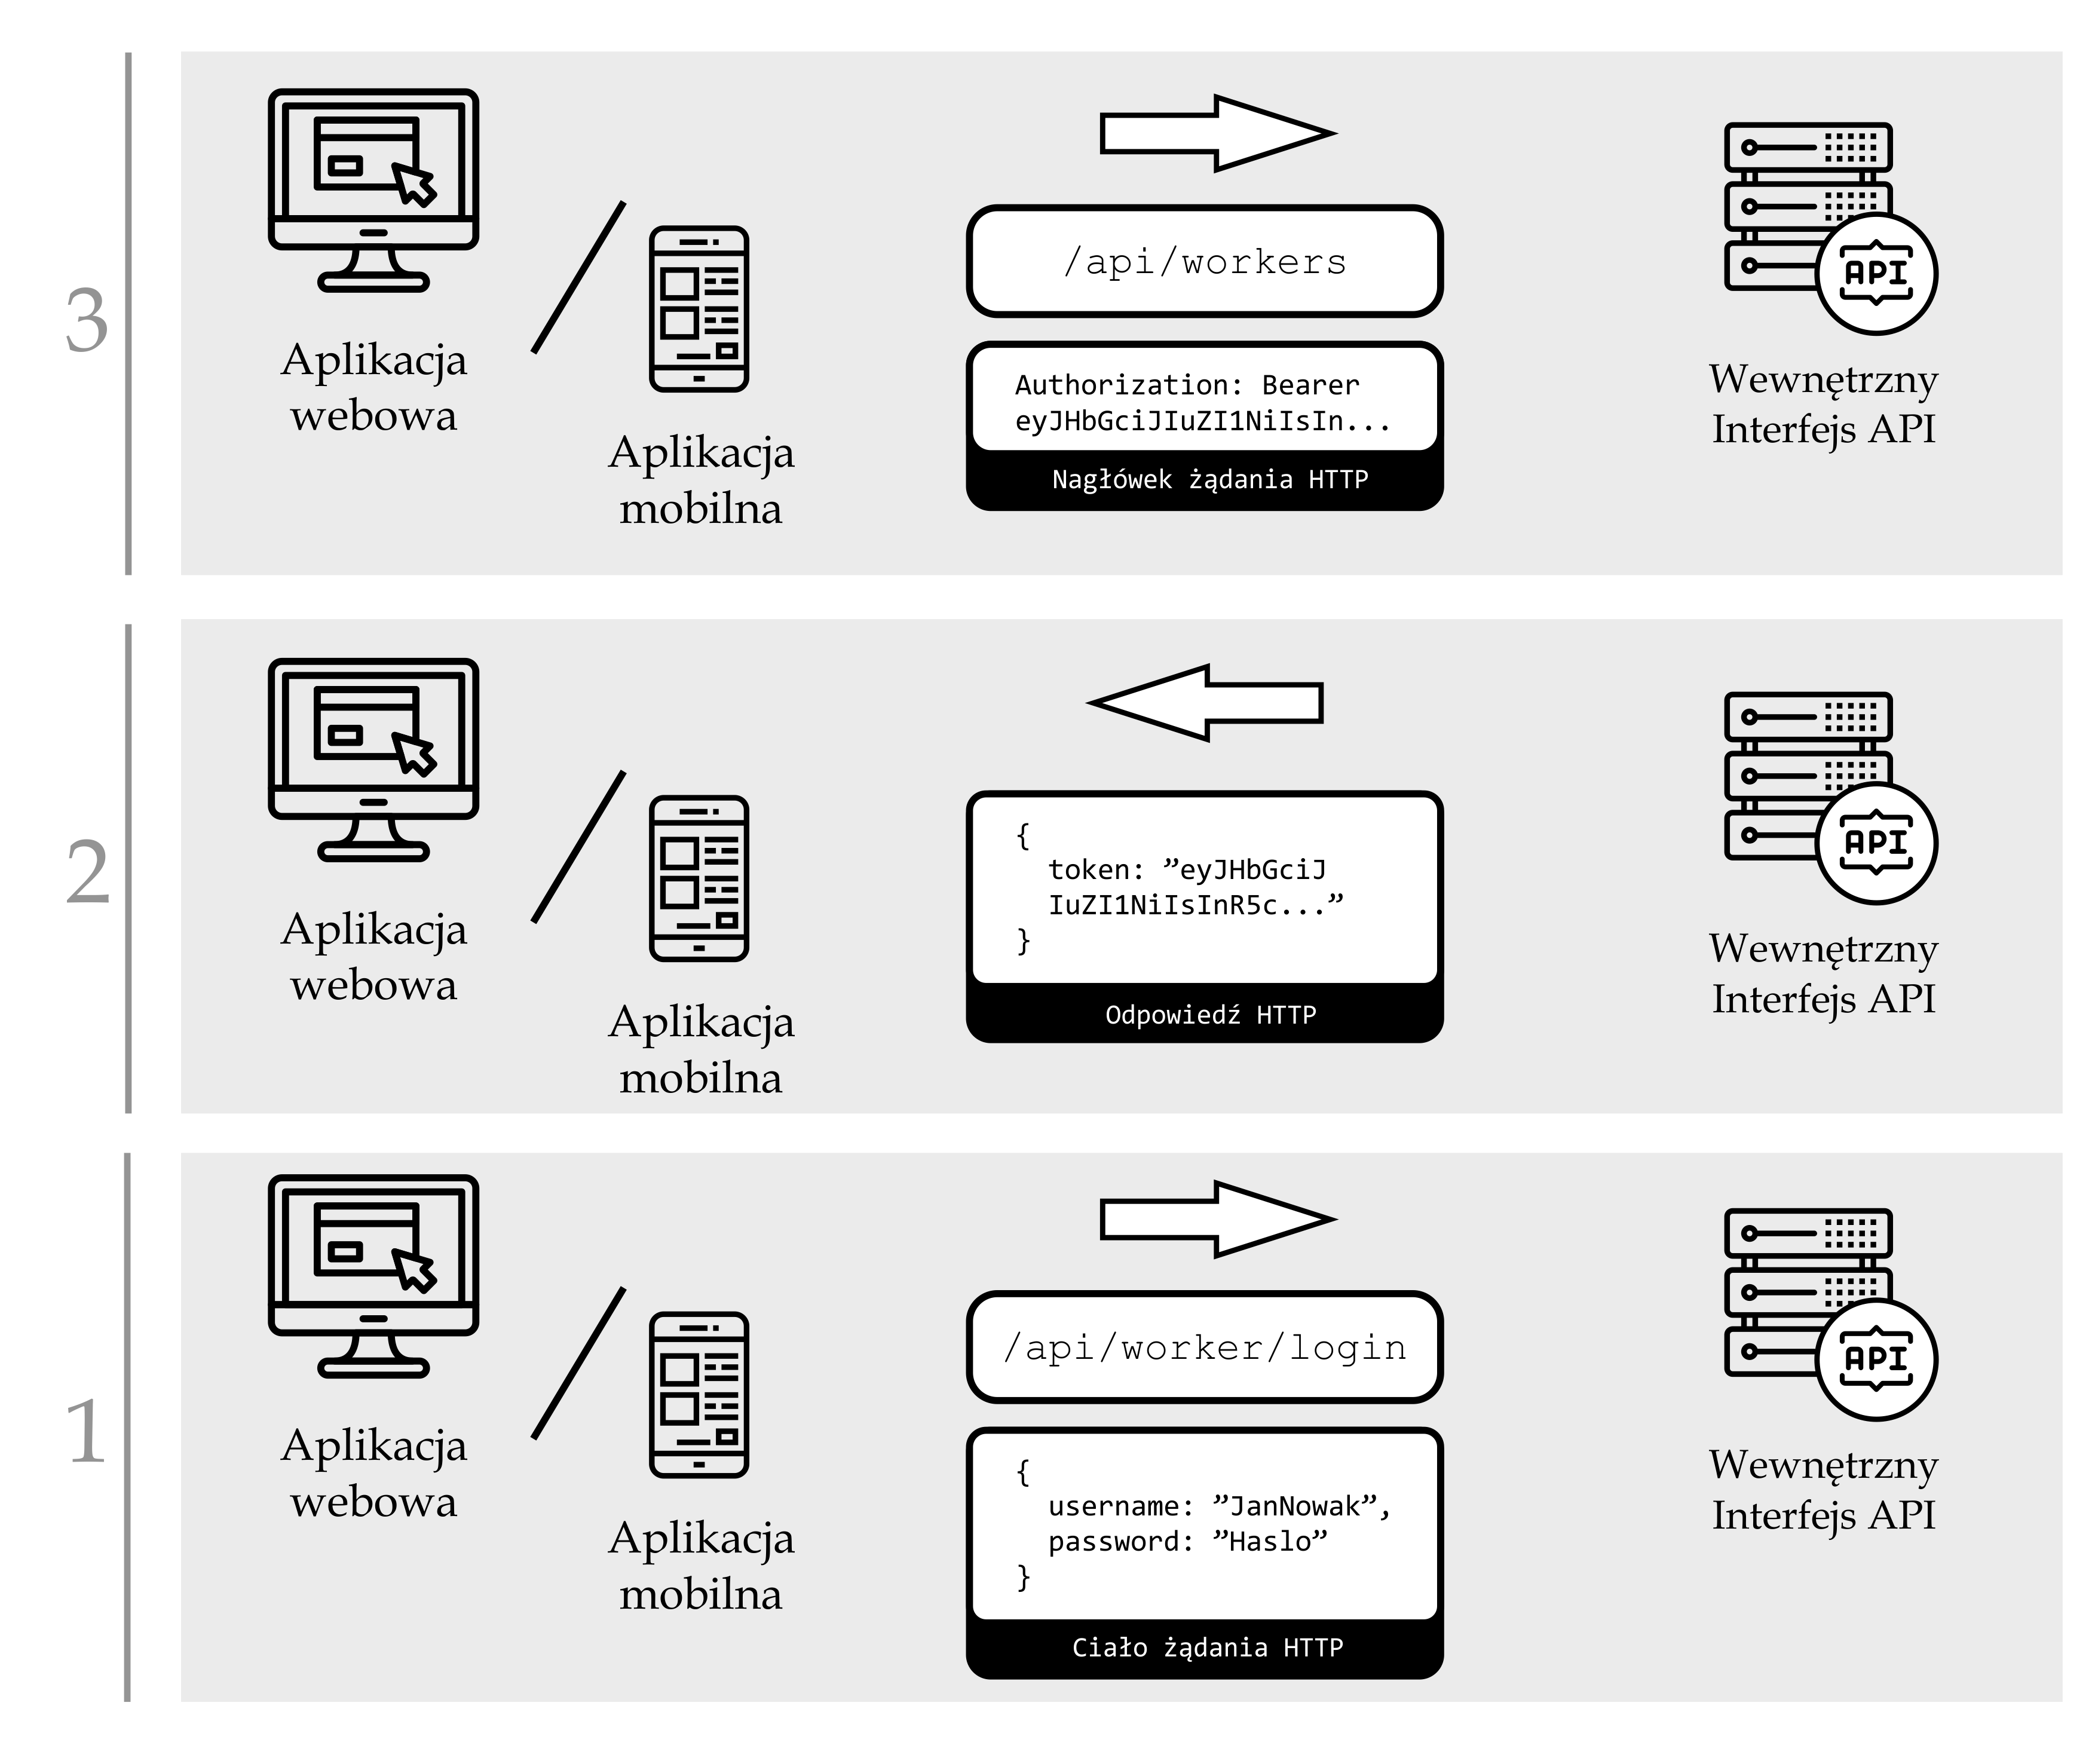
\includegraphics[width=0.6\linewidth]{rys03/uwierzytelnianie-autoryzacja}
 \caption{Proces uwierzytelnienia oraz autoryzacji użytkownika przed interfejsem API}
 \label{fig:uwierzytelnienie-autoryzacja}
\end{figure}


\subsection*{Segregacja zapytań oraz komend w kontekście odwołań do źródła danych}
\subsection*{Konwencja REST}


\section{Testowanie usług sieciowych}
\section{Wykorzystywane technologie}
\section{Przegląd literatury}
W niniejszym rozdziale przedstawione zostaną pozycje literaturowe, do których odnosić się będzie opisywana praca dyplomowa. Pozycje te, podzielone zostały na oddzielne grupy, związane z określoną tematyką.

Na początku, przedstawiona zostanie literatura powiązana z aspektem budowy interfejsów programowania aplikacji oraz będąca wprowadzeniem do wykorzystywanych technologii. Następnie, opisane zostaną pozycje traktujące o wydajności interfejsów API, a także o analizie działania powszechnie dostępnych serwisów internetowych opartych o metodologię REST. Kolejne prace, skupiać się będą na tematyce testowania usług sieciowych, teorii testowania, a także konfiguracji narzędzi dla testów rozproszonych. W następnej kolejności, wspomniane zostaną prace naukowe oraz dokumenty standaryzacyjne dotyczące sposobu działania protokołu przesyłania danych hipertekstowych. Ostatnią grupą pozycji literaturowych będą prace referencyjne dotyczące badań wydajności systemów internetowych.

Pozycja [1] stanowi wprowadzenie do zaawansowanych konceptów języka C\#, a także dostarcza informacji związanych z wykorzystaniem tego języka w środowiskach uruchomieniowych .NET oraz .NET Core. W początkowych rozdziałach przedstawiono sposób budowy, kompilacji oraz wykonywania programu w środowisku .NET. Kolejno opisana została struktura bazowych aplikacji uruchamianych w tym właśnie środowisku i tworzonych za pomocą języka C\#. Ostatnim elementem wprowadzenia do opisywanej technologii było przedstawienie struktur języka w kontekście obiektowego paradygmatu programowania.    W następnych sekcjach literatury, w sposób wyczerpujący poruszono tematykę bardziej zaawansowanych aspektów programowania w języku C\#, którymi są między innymi: kolekcje i typy generyczne, delegaty i wyrażenia lambda, czy też cykl życia obiektu w pamięci programu. Ważnym tematem, poruszonym w ramach tej książki jest struktura oraz zasada działania środowiska .net core, będącego podstawowym elementem interfejsów programowania aplikacji tworzonych w języku C\#.

Analogiczną do przedstawionej powyżej pozycji literaturowej, dotyczącą jednak technologii NodeJS oraz języka JavaScript jest [2]. W ramach tej pracy zawarto obszerne wprowadzenie do platformy NodeJS uwzględniające ponadto kwestie obsługi operacji wejścia/wyjścia, wykonywania natywnego kodu JS, czy też przetwarzania operacji przez silnik NodeJS oraz bibliotekę libuv. Znaczna część pracy, obejmuje przedstawienie zaawansowanych wzorców projektowych, których głównym przeznaczeniem jest obsługa zdarzeń oraz operacji asynchronicznych. Wspomniane zostały także rozwiązania dotyczące skalowalności aplikacji z wykorzystaniem mechanizmów kolejkowania wiadomości.

Niezależnie od wykorzystywanej technologii, interfejsy programowania aplikacji, które zostały zbudowane na potrzeby tej pracy dyplomowej, oparte są o styl architektoniczny RESTful. Styl ten, jest pewnym zbiorem zasad projektowania usług sieciowych, określającym zarówno aspekty sposobu komunikacji klienta z usługą sieciową, jak i techniczne wymagania dotyczące przetwarzania żądań. Dobre praktyki, które uwzględnia metodologia REST, zawarte zostały w pozycji literaturowej [3]. Autorzy tego dokumentu, na wstępie dokonują porównania architektury zorientowanej na zasoby, będącej podstawą konwencji REST, z popularną uprzednio architekturą zorientowaną na usługi. Następnie, przedstawiane są najlepsze praktyki, cele oraz reguły REST dotyczące projektowania interfejsu programowania aplikacji. Co więcej, w omawianej książce zawarte zostały także podstawowe oraz zaawansowane wzorce projektowania API, uwzględniające aspekty bezstanowości, paginacji, osiągalności, a także identyfikacji zasobów interfejsu. Końcowe rozdziały książki, wprowadzają w kwestie testowania oraz bezpieczeństwa REST API, omawiają technikę kompozycji usług RESTful, a także przedstawiają rozwiązania (biblioteki oraz języki programowania) pozwalające na tworzenie interfejsów API zgodnych z metodologią REST.

Podstawowym celem działania interfejsu programowania aplikacji jest dostarczenie danych do konsumenta, bądź też ich manipulacja zgodnie z jego żądaniem. Aby operować na danych, interfejs API musi komunikować się ze źródłem danych, którym najczęściej jest serwer bazodanowy. W celu dostarczenia metod komunikacji pomiędzy API a źródłem danych, które jednocześnie są niezależne od wykorzystywanego źródła, a także pozwalają na zarządzanie danymi z poziomu struktur języka, stworzone zostały biblioteki zwane maperami obiektowo-relacyjnymi (ang. Object-Relational Mappers). Dla API napisanego w języku C\# podstawowym rozwiązaniem ORM jest biblioteka Entity Framework Core, która przedstawiona została w pozycji [4]. Pozycja ta, uwzględnia zarówno opis działania najczęściej wykorzystywanych metod służących do manipulacji danymi, jak i rolę klasy kontekstu bazodanowego w procesie tłumaczenia operacji programistycznych na polecenia bazodanowe. Ponadto, dowiedzieć możemy się jak przetwarzać zaawansowane typy danych (takie jak np. DateTime), czy też w jaki sposób wykorzystywać zapytania LINQ do budowania kwerend.

Dla interfejsu programowania aplikacji napisanego w języku JavaScript i uruchamianego w środowisku NodeJS, w przeciwieństwie do platformy .NET, zastosować możemy zdecydowanie większą liczbę bibliotek pełniących rolę maperów obiektowo-relacyjnych. Biblioteki te, zostały opisane w pozycjach [5] i [6]. Pozycja [5] pełni rolę całościowego wprowadzenia do tematyki tworzenia interfejsów API, korzystając z platformy NodeJS, frameworka ExpressJS oraz nierelacyjnej bazy danych MongoDB. Rodział piąty tej pracy, traktujący o wykorzystaniu baz danych NoSQL, przybliża tematykę jednego z najczęściej wykorzystywanych maperów obiektowo-relacyjnych dla Node czyli mongoose. Przedstawiono tutaj sposób zestawienia połączenia z serwerem bazodanowym, tworzenia encji modelu, przekształcanego następnie na struktury bazy danych, a także wykonywania operacji dostępu do danych i ich modyfikacji. W pracy [6] natomiast, porównano nierelacyjne podejście do składowania danych typu geograficznego z podejściem relacyjnym, wykorzystując w tym przypadku biblioteki mongoose i sequelize. Oba mapery obiektowo relacyjne zostały użyte w ramach interfejsu API wykorzystującego technologie NodeJS/ExpressJS. Celem opisywanej pracy było przedstawienie różnic w czasach odpowiedzi API na uzyskane żądanie, dla różnej liczby danych geolokalizacyjnych, uwzględniając zastosowanie relacyjnych i nierelacyjnych baz danych.

Następne pozycje literaturowe, związane są z analizą usług REST oraz wydajnością webowych interfejsów programowania aplikacji.

Pozycja [7] stanowi analizę 500 serwisów internetowych z listy alexa.com4000 najpopularniejszych dostępnych publicznie usług sieciowych. Twórcy każdego z 500 serwisów deklarują zgodność swoich produktów z konwencją REST. Przeprowadzona analiza dotyczyła kluczowych aspektów technicznych związanych z funkcjonowaniem API, stopnia zgodności API z regułami dotyczącymi metodologii REST, a także przestrzegania najlepszych praktyk projektowania interfejsów programowania aplikacji, takich jak m.in. zastosowanie mechanizmu wersjonowania. W trakcie analizy, zaobserwowano określone trendy dla aplikacji REST API, takie jak m.in. rozpowszechnione wsparcie notacji JSON, czy wykorzystywanie narzędzi do dokumentacji generowanej programowo. Ponadto, zauważono, że tylko ok. 0.8\% analizowanych serwisów webowych przestrzega w sposób ścisły reguł zawartych w ramach konwencji REST.

Wydajność interfejsów programowania aplikacji, jako jeden z elementów miary jakości API została przedstawiona w pozycji [8]. Na początku pracy, jej autorzy wskazują na interakcję interfejsu programowania aplikacji z systemami klienckimi. Opisany został tutaj zestaw protokołów sieciowych wykorzystywanych podczas formułowania i transmisji żądania, system zunifikowanych lokacji zasobów, a także semantyka interakcji w zależności od wykorzystywanych typów żądań protokołu hipertekstowego. Ponadto, wskazano najczęstsze przyczyny błędów przepływu danych dla http, uwzględniając działanie usługi DNS, błędy połączenia, błędy leżące po stronie klienta, a także błędy wynikające z działania serwera. Kolejna część pracy, związana jest ze składowymi metryki jakości, do których według autorów, poza wydajnością, zaliczyć możemy: dostępność, procent żądań dla których uzyskano pozytywną odpowiedź, osiągalność, a także możliwość sprawdzenia stanu usługi w dowolnym momencie jej działania. Dodatkowo, w niniejszej pracy zaproponowano podejście oraz zestaw narzędzi pozwalających na dokonanie ewaluacji jakości interfejsu programowania aplikacji, zgodnie z przyjętą normą jakości.

Kolejnym etapem następującym po zdefiniowaniu metryki wydajności, jest ustalenie wartości tejże metryki w kontekście testowanych usług sieciowych. Przytoczone poniżej pozycje literaturowe, związane są z wykonywaniem pomiarów wydajności API, czyli testowaniem.

Pozycja [9] stanowi obszerne wprowadzenie do teorii testowania oprogramowania. W pierwszych rozdziałach tego dokumentu, wyjaśniono czym jest testowanie, dlaczego jest ono niezbędne podczas tworzenia oprogramowania, a także jak wygląda podstawowy proces wykonywania testów. Następnie przedstawiono proces testowania w kontekście tworzenia oprogramowania. Uwzględniono tu zarówno modele cyklu życia rozwoju systemów w powiązaniu z testowaniem, poziomy realizowanych testów, ich typy, jak i sposoby zarządzania testami. Kolejne rozdziały tyczą się testowania statycznego (tj. testowania funkcjonalności lub modułu na poziomie jego specyfikacji lub implementacji bez wykonywania kodu testowanego oprogramowania), dostarczają teorii związanej z poszczególnymi technikami testowania rozwiązań oraz przedstawiają aspekt organizacji, planowania, monitorowania oraz uwzględniania ryzyka w czasie dokonywania ewaluacji systemów. W ostatnim z rozdziałów dokumentu, autorzy przedstawiają narzędzia przydatne w procesie testowania, a także sposób ich efektywnego wykorzystania w codziennej pracy.

Pozycja [10] zawiera wiele analogicznych treści do pracy opisanej powyżej, jednakże rozwija ona w sposób wyczerpujący, wspomniane tylko w poprzedniej pracy aspekty. W części drugiej dokumentu zawarto dogłębną analizę zagadnienia testowania statycznego, uwzględniając m.in. testowanie zgodności ze standardami oprogramowania, symboliczne wykonywanie kodu, a nawet wprowadzając aparat matematyczny do formalnego dowodzenia poprawności fragmentów oprogramowania. W ramach tej książki, przedstawiono także dynamiczną analizę systemu (tj. testowanie funkcjonalności lub modułu na poziomie wykonywanego kodu) uwzględniając często występujące błędy związane m.in. z nieumiejętnym zarządzaniem strukturami pamięci programu. Ponadto, uwzględniono zagadnienie priorytetyzacji przypadków testowych, wprowadzając pojęcie miary średniego procenta wykrytych usterek. Autor dokumentu przedstawia także testowanie charakterystyk jakościowych zgodnie z normą ISO 9126 oraz ISO 25010, tworzenie dokumentacji w ramach zarządzania testowaniem, czy chociażby zarządzanie incydentami występującymi w ramach procesu ewaluacji oprogramowania.

W ramach pozycji [11], dowiedzieć możemy się ponadto o testowaniu usług internetowych. Przedstawiono tutaj podstawową strukturę standardowej usługi sieciowej (w tym przypadku – usługi e-commerce) cechującej się architekturą trójwarstwową. Ponadto, wyjaśniono rolę każdej z warstw systemu, a także przedstawiono aspekty testowania oprogramowania w kontekście każdej z nich. Dodatkowo, zawarte zostały przykładowe przypadki testowe, dotyczące zarówno prezentacji danych w systemie, jak i dostępu do danych poprzez serwer webowy. Dla zaprezentowanych przypadków testowych, przedstawione zostały także scenariusze realizacji testów w postaci listy czynności jakie należy podjąć, aby dokonać ewaluacji systemu.

Aspekty technologii testowania oprogramowania ujęte zostały także w pozycji [12]. Artykuł ten, stanowi sekcję wprowadzającą do książki pt. Tutorial: Software Testing and Valdation Techniques, tego samego autora. Pozycja ta, przedstawia przekrój technik oraz technologii testowania oprogramowania wykorzystywanych na przestrzeni ostatnich ok. 30 lat. Opisane zostały tutaj zarówno teoretyczne podstawy testowania, narzędzia i techniki analizy statycznej i dynamicznej, oceny efektywności przeprowadzanych testów, a także badania przeprowadzane w dziedzinie testowania i walidacji oprogramowania. Omawiany artykuł, wyszczególnia pozytywne oraz negatywne aspekty poszczególnych technik oraz wskazuje przydatność określonych rozwiązań do testowania oprogramowania różnego typu.

Ostatnią przytoczoną w ramach tego przeglądu literaturowego pozycją, dotyczącą teorii ewaluacji oprogramowania jest [13]. Pozycja ta, stanowi normę międzynarodowej organizacji normalizacyjnej (ang. International Organization for Standardization) dotyczącą weryfikacji jakości oprogramowania. Uwzględniono tu przede wszystkim znaczenie pojęć stosowanych w dziedzinie testowania oprogramowania, wprowadzono definicje dla określonych terminów oraz zjawisk występujących w ramach ewaluacji systemów, a także określono zgodność wprowadzanych przez standard konceptów, z konceptami zawartymi w standardach pochodnych. Główną część dokumentu, stanowi wprowadzenie szkieletu modelu jakości, uwzględniającego określone modele jakościowe, modele jakości w użyciu, a także modele jakości produktu. Dodatkowo, przedstawiono cel oraz sposób wykorzystania modeli jakościowych, wyjaśniono różnicę w postrzeganiu modeli jakościowych z punktu widzenia różnych interesariuszy, a także zdefiniowano relacje pomiędzy określonymi modelami. Dokument ten, wraz z normą ISO 9126, stanowią definicję pojęcia jakości w kontekście testowania oprogramowania.

Pozycja [14] stanowi przegląd narzędzi wykorzystywanych do testowania działania systemów komputerowych. Na początku książki, wprowadzany jest termin zapewnienia jakości (ang. Quality Assurance), który w dzisiejszych czasach definiuje zakres odpowiedzialności osoby testującej oprogramowanie. Kolejno, przedstawiane są kryteria sukcesu dotyczące tworzonego systemu, a także fazy poszczególnych modeli rozwoju oprogramowania zorientowanych na procesy. Analogicznie do pozycji literaturowych przedstawionych uprzednio, w ramach tej pozycji określone zostały metryki i definicje jakości oprogramowania oraz omówiony został proces realizacji testów. Główna część omawianego dokumentu skupiona jest wokół narzędzi stosowanych do realizacji ewaluacji oprogramowania. Wyszczególniono tutaj narzędzie WinRunner, przedstawiając między innymi wykorzystywany w tym programie skryptowy język testów (ang. Test Script Language). Ponadto, przedstawiono architekturę oraz najważniejsze funkcjonalności narzędzi SilkTest, SQA Robot, LoadRunner, TestDirector, QuickTest Professional a także Apache JMeter. Ostatni z wymienionych programów, wykorzystywany zostanie w ramach niniejszej pracy dyplomowej, dlatego też dalszy przegląd tej pozycji literaturowej skupiony będzie na rozdziale dotyczącym właśnie tego narzędzia. Opis funkcjonalności aplikacji JMeter został w niniejszej pozycji podzielony na sekcje związane z testowaniem rozwiązań bazodanowych wykorzystujących interfejs JDBC (ang. Java DataBase Connectivity), a także sekcję dotyczącą testowania aplikacji bazujących w swoim działaniu na protokole hipertekstowym. Przedstawiono tutaj sposób tworzenia grup wątków reprezentujących użytkowników aplikacji, generowania żądania protokołu hipertekstowego, uruchomienia mechanizmu nasłuchiwania na odpowiedź serwisu, dodawania licznika czasu, a także zapisywania i przeglądania rezultatów przeprowadzonego testu.

W ramach dokumentów [15] oraz [16] przedstawiono pełen zakres funkcjonalności dostępnych w ramach narzędzia Apache JMeter. Pierwsza z prac (tj. [15]), skupia się na wykorzystaniu narzędzia w celu wykonywania testów wydajności usług sieciowych, natomiast druga z pozycji (tj. [16]), przedstawia aplikację JMeter dla różnych kontekstów jej potencjalnego użycia. W obu pracach wyszczególnione zostają podstawowe elementy, na które składa się środowisko testowe. Elementami tymi są: grupy wątków, komponenty próbkujące, kontrolery, komponenty nasłuchujące, liczniki czasu oraz asercje. Ponadto,  omówiono elementy graficznego interfejsu użytkownika dla aplikacji, przedstawiono proces instalacji oraz uruchamiania narzędzia JMeter, a także zdefiniowano pojęcie planu testów. W kontekście pracy [15], poza wymienionymi uprzednio kwestiami, zobrazowany został także proces wykonywania testu przeciążeniowego dla usługi zorientowanej na serwisy (ang. Service-Oriented Application). Proces ten uwzględniał: tworzenie grupy wątków, konfigurację struktury żądania wysyłanego do usługi, uruchomienie testu, a także pozyskanie wyniku. W pracy [16] natomiast, analogiczny proces, możemy zaobserwować dla monolitycznej aplikacji internetowej oraz interfejsu programowania aplikacji. Ponadto, przedstawione zostały zaawansowane opcje konfiguracji elementów nasłuchujących oraz liczników czasu, a także pokazany został proces wykorzystania pośredniczącego serwera http, w celu dokumentowania realizowanych żądań.

Następne pozycje literaturowe omówione w ramach tej pracy, dotyczą budowy oraz zasady działania internetowego protokołu hipertekstowego (ang. Hypertext Transfer Protocol), a także implementacji mechanizmu zarządzania stanem. Mechanizm ten, w związku z naturą protokołu http, nie jest w nim domyślnie realizowany.

Pozycja [17] stanowi techniczny dokument dotyczący semantyki oraz budowy internetowego protokołu hipertekstowego w wersji 1.1. Zdefiniowano w nim pojęcie zasobu żądania oraz omówiono cykl życia jego przetwarzania. Wskazano także moment, w którym zasób rekonstruowany jest przez serwer na podstawie jego efektywnego identyfikatora URI (ang. Uniform Resource Identifier). Ponadto, nakreślono pojęcie reprezentacji danych przesyłanych za pomocą protokołu http, definiując określone pola nagłówkowe dotyczące: typu danych, sposobu kodowania, języka danych, a także lokalizacji zasobu. Kolejne rozdziały dokumentu zawierają informacje dotyczące definicji dozwolonych metod protokołu http oraz znaczenia jakie te metody wprowadzają w kontekście operacji na zasobie. W dokumencie przedstawiono także kody statusu odpowiedzi na żądnie, grupując je w sposób semantyczny. Dla każdego z przedstawionych kodów statusu nakreślono kontekst, w jakim odpowiedź, oznaczona tym właśnie kodem, powinna być zwracana klientowi. Na końcu pracy, omówiono kwestie związane z bezpieczeństwem protokołu takie jak: ataki bazujące na wstrzykiwaniu kodu czy ochrona przed ujawnianiem informacji wrażliwych w identyfikatorach zasobów.

Pozycja [18] pozwala na poszerzenie wiedzy dotyczącej protokołu hipertekstowego w bardziej praktycznym kontekście. Podobnie jak w dokumencie [17], przedstawiono tutaj informacje teoretyczne dotyczące architektury protokołu, definicji zasobów czy też ujednoliconego formatu ich adresowania. Ponadto, wskazano i scharakteryzowano określone typy połączeń realizowanych z wykorzystaniem protokołu hipertekstowego. Co więcej, dla każdego z nich rozważono kwestie związane z wydajnością połączenia pomiędzy klientem a serwerem. Kolejne rozdziały pracy [18] traktują o identyfikacji klienta w ramach serwera, jego uwierzytelniania przed serwerem, a także szyfrowania danych przesyłanych pomiędzy tymi dwiema jednostkami.  W niniejszej pracy wspomniano także o internacjonalizacji żądań w kontekście zastosowania nagłówka ‘Accept-Language’. Ostatnie rozdziały dokumentu dotyczą kwestii publikowania i dystrybucji zawartości. Wyszczególnione zostały tu takie elementy jak: web hosting, systemy publikacji treści, czy też mechanizm przekierowań oraz równoważenia obciążeń.

Zgodnie z charakterystyką protokołu http, realizuje on komunikację w sposób bezstanowy. Oznacza to, że domyślnie, pomiędzy klientem a serwerem nie jest utrzymywana sesja połączeniowa, a każde żądanie generowane przez klienta w kierunku serwera rozpatrywane jest indywidualnie. Rozwiązanie takie, pozwala na znaczące przyspieszenie działania protokołu hipertekstowego, a także uproszczenie jego konstrukcji. Jednakże, szczególnie w przypadku aplikacji internetowych komunikujących się z serwerem http, bezstanowy charakter protokołu bywa problematyczny w aspekcie kontekstu wysyłanych sekwencyjnie żądań. Dlatego też, do protokołu http wprowadzono mechanizm zarządzania stanem opisany w dokumencie [19]. Dokument ten, definiuje pola nagłówkowe o nazwach ‘HTTP Cookie’ oraz ‘Set-Cookie’. Pola te, mogą być używane przez serwery http w celu przechowywania stanu w ramach aplikacji klienckich, dając serwerom tym możliwość zarządzania, zawierającą stan sesją, przy wykorzystaniu protokołu bezstanowego. W niniejszym dokumencie, dla obu przedstawionych pól wyszczególniono atrybuty składowe pola, a także określono znaczenie każdego z nich. Ponadto, dokument definiuje wymagania dla klienta http, dotyczące możliwości wykorzystania mechanizmu zarządzania stanem. Pod uwagę wzięte zostały także kwestie bezpieczeństwa takie jak identyfikatory sesji, słaba poufność danych, czy też zaufanie do usługi nazw domenowych w celu prawidłowego działania mechanizmu zarządzania stanem.

Ostatnia grupa pozycji literaturowych, zawartych w ramach niniejszego przeglądu literaturowego dotyczy badań związanych z testowaniem wydajności aplikacji internetowych w środowisku rozproszonym. Pozycje przedstawione poniżej, będą stanowić prace referencyjne względem niniejszej pracy dyplomowej.

Artykuł [20] dotyczy porównania wydajności działania interfejsów programowania aplikacji tworzonych z wykorzystaniem platform .NET Core 3.1 oraz .NET 5. Celem powstania tego dokumentu była weryfikacja zjawiska wzrostu wydajności działania programów, tworzonych i uruchamianych z wykorzystaniem nowszej z platform firmy Microsoft. Praca ta, ma także na celu pomóc pozwolić odpowiedzieć na pytanie, czy kod źródłowy interfejsu programowania aplikacji o określonych funkcjonalnościach, a także korzystający z określonych narzędzi, powinien zostać zaktualizowany w taki sposób, aby wspierać najnowszą, stabilną wersję środowiska .NET. W ramach dokumentu, w celu realizowania pomiarów wydajności wykorzystano opisane w poprzednich akapitach narzędzie Apache JMeter, a także dedykowaną środowisku .NET, bibliotekę BenchmarkDotNet. Kolejne rozdziały artykułu przedstawiają przygotowane środowisko testowe, plan wykonywanych testów, a także uzyskane rezultaty wraz z ich analizą. Autor pracy, zobrazował wyniki sześciu testów wydajnościowych, biorących pod uwagę proces serializacji oraz deserializacji obiektów typu JSON za pomocą bibliotek NewtonsoftJson, a także System.Text.Json. Ponadto, przygotowany został test wyszukiwania wzorca z obszernym ciągu tekstowym oraz test wykorzystania punktu końcowego jako klienta zewnętrznego API. Na podstawie otrzymanych rezultatów, wnioskować możemy o około 24 procentowym średnim wzroście wydajności wykonywania operacji realizowanych w ramach testów. Ponadto, wykazano także dość znaczący (około 35 procentowy) średni spadek wydajności nowego rozwiązania względem poprzednika, w kontekście testów obciążeniowych.

Analogiczne badania przeprowadzono w ramach pracy [21]. W tym przypadku jednak, nie skupiały się one na aspekcie porównania technologii, a na sposobie wykonywania pomiarów, a także definiowaniu kryteriów oceny jakości. W pracy tej, interfejs programowania aplikacji zbudowany w oparciu o metodologię REST poddawany był zmiennym obciążeniom (tj. testy linii bazowej, testy obciążeniowe oraz testy przeciążeniowe). W czasie dokonywania ewaluacji monitorowano średni czas odpowiedzi serwera, zgodność kodów statusu zawartych w ramach uzyskiwanych odpowiedzi, informacje o zużyciu zasobów sprzętowych serwera, czy też wartość wskaźnika satysfakcji klienta. Rezultaty przeprowadzonych badań wykazały kluczowe znaczenie optymalizacji kodu źródłowego aplikacji, w kontekście realizacji rozbudowanych i skalowalnych usług sieciowych.
